\chapter[K-mer Counting]{K-mer Counting and K-mer Abundance Histograms}

A $K$-mer is a substring of length exactly~$k$. In \emph{$k$-mer counting} we take sequencing reads as an input and we want to know for each $k$-mer occurring in the reads, how many occurrences does it have. We can summarize the counts of all $k$-mers, in a $k$-mer histogram.
The \emph{$k$-mer abundance histogram $H_k$ (shortly the $k$-mer histogram)} is an array, where the $i$-th element (denoted by $H_k[i]$) is the number of unique $k$-mers occurring in the data exactly $i$ times. The size of the histogram denoted by $|H_k|$ is maximal $i$ such that $H_k[i] > 0$.

Counting of the $k$-mer occurrences is one of the key problem in many applications in bioinformatics.
For example, it was used to separate several individual
genomes when sequencing a metagenomic mixture of different microbes isolated from a certain environment~\cite{Wu2011, Wang2012}.
It is also used in error correction algorithms e.g.\ for correcting errors prior the DNA assembly~\cite{Pevzner2001}, sequence aligners~\cite{edgar2004muscle} and repeat detectors~\cite{caponnetto2013efficiency}.
Moreover, it is suitable for various sequence read analyses and genome size estimation~\cite{covest, williams, waterman}.
For some of these applications, computation of the $k$-mer abundance histogram is sufficient.
In particular, we will use the $k$-mer histograms in~Chapter~\ref{chap:genomesize} for estimating the coverage and the size of a genome.

A typical NGS data set, consists of many reads. Although these reads typically cover the target genome multiple times, sequencing errors in the reads result in many unique $k$-mers.
This causes a high memory usage of naive approaches to the problem of $k$-mer counting or $k$-mer histogram computation.
For example the 100Mb long genome with no repeats, sequenced with $50\times$ coverage, read length 100, and error rate $1\%$ contains approximately $4\cdot 10^9$ unique 21-mers. Just to store a counter for each of them, we need approximately $40$ GB of memory. For larger genomes (e.g.\ 3.2Gb long human genome, or 16Gb onion (Allium cepa) genome), much more memory would be needed.

There are several existing tools addressing this issue, for example Tallymer~\cite{tallymer}, JELLYFISH~\cite{jellyfish}, BFCounter~\cite{bfcounter}, DSK~\cite{dsk} and Khmer~\cite{khmer}. Each tool must handle the trade-off between speed, memory usage, disk usage, precision and random access capability. Most approaches to the $k$-mer counting problem use hash tables, Bloom filters or suffix arrays.
The tools have various limitations --- for example DSK does not provide random access to the counts and Khmer does not count $k$-mers exactly.
The comparison of the tools can be found in~\cite{khmer}.

\section{Simple Hashing Approach}

Let us first briefly explain the naive solution, so that we can extend and compare it to the methods used in selected published tools.
Suppose we want to count occurrences of $k$-mers in sequence $S$.
We create a hash table $T$, in which $k$-mers will be keys and their counts stored as values, and then scan the sequence $S$.
At each position $i$, we take the $k$-mer $K_i$ corresponding to that  position, compute $hash(K_i)$ and increase the corresponding item in the table, after handling possible collisions.

We can then query the hash table for the number of occurrences of a~particular $k$-mer, or iterate through the whole table to compute the histogram.

For small genomes with very low sequencing error rate, this approach is sufficient. However, higher error rate produces more unique $k$-mers and together with large genomes makes the hash table so big it does not fit in computer's memory. In addition, the general hash table is not parallelizable, which makes this approach slow.

\section[Filtering Unique K-mers]{Filtering Unique K-mers Using Bloom Filters}

Error rate in Illumina sequencing machines is usually about 1--5\%. However, even at $1\%$, the probability that a 20-mer contains an error is $1 - 0.99^{20} \approxeq 0.18$; i.e.\ about 18\% of $k$-mers from a given position in DNA will differ from the correct $k$-mer. It means that if we read a particular $k$-mer for example $20\times$ and two of them are erroneous, we would get three different $k$-mers, from which two of them would have abundance one and one would have abundance 18.

In general, the correct $k$-mers abundances are distributed according to the Poisson distribution with mean $c'$, where $c'$ is an average number of correct $k$-mers covering a single position in a genome (see Chapter~\ref{chap:genomesize} for more details). In low to middle coverage, the most erroneous $k$-mers contribute to the abundance of one.
Therefore, we get most $k$-mers unique in low to middle coverage data.

If we do not store these unique $k$-mers in the hash table, we can save a lot of memory. We can use a more memory efficient, probabilistic data structure called \emph{Bloom filter}~\cite{bloomfilter} to store the unique $k$-mers.

The Bloom filter stores a set of elements (in our case $k$-mers), and it supports two operations: \method{add} for adding an element to the set and \method{test} for testing whether an element is in the set. The following property holds for the \method{test} operation:
\begin{itemize}
  \item If the element is in the set, test returns \emph{true}.
  \item If the element is not in the set, test returns \emph{false} with a high probability.
\end{itemize}
If the test method returns true, the element is probably in the set, otherwise it is definitely not there.

A Bloom filter consists of a bit vector of length $n$ and $m$ hashing functions, each transforming the element to the position in the bit vector. The parameters $n$ and $m$ directly affect the false positive rate of the Bloom filter.
The \method{add} operation computes $m$ positions from $m$ hashing functions applied to the element and sets all corresponding bits in the vector to one.
The \method{test} operation computes $m$ positions from the element and checks whether each of them is set to one. If any of them is zero, it returns false, otherwise it returns true. Further details are described in~\cite{bloomfilter}.

We can use a Bloom filter to store all $k$-mers we have seen at some point of the computation. We just add every $k$-mer to the Bloom filter during the computation. Before adding the $k$-mer, we first check if the $k$-mer is already in the Bloom filter. If yes, it means that we have probably seen this $k$-mer before, and we also add it to the hash table with the starting count 2. In this way we get approximate counts for each $k$-mer.
With one more pass through the input data we can get exact counts.
Any input $k$-mer, which is not in the hash table is certainly unique, and the counts of $k$-mers in the hash table can be also recomputed. This approach was used in BFCounter~\cite{bfcounter}.

\section[Probabilistic K-mer Counting]{Probabilistic K-mer Counting Using Count-Min Sketch}

The Count-Min sketch~\cite{countminsketch} data structure enables counting objects in sublinear space. It supports two operations:
\begin{itemize}
  \item \method{incrementcount(x)} %chktex 36
  \item \method{getcount(x)} %chktex 36
\end{itemize}

The data structure consists of $m$ hash tables with different hash functions.
The \method{incrementcount(x)} operation computes a hash of $x$ using each hash function and increments the corresponding counters in all hash tables. The \method{getcount} operation computes hash of $x$ using each hash function and takes the minimum of all corresponding values in hash tables as the result. %chktex 36

If there is a collision in each table for a particular object, the \method{getcount} operation may return greater value for such object. This false positive rate depends on the collision probability, which decreases with increasing number of hash tables and their sizes.

This data structure can be directly used to the $k$-mer counting problem. As it does not store the $k$-mers themselves, it allows in memory $k$-mer counting and querying, which is useful for streaming applications.
More details about false positive rate estimation and comparison to other approaches for $k$-mer counting can be found in~\cite{khmer}.

\section[Other Improvements]{Other Improvements of the Hashing Approach}

The basic hashing approach to $k$-mer counting can be further improved in various ways; here we describe two such improvements.

\paragraph{} The first is a memory usage improvement using an explicit disk-memory trade-off. The \emph{Disk Streaming of K-mers (DSK)} algorithm~\cite{dsk} exploits the fact that the multi-set of $k$-mers can be partitioned, and each partition can be loaded to the memory separately.

The algorithm has two parameters: the memory size $M$, and the disk space $D$ expressed in bits. During the computation, the algorithm does not exceed the memory and disk space constraints given by the parameters.

The algorithm works in several iterations, which number is proportional to the memory needed to store all the $k$-mers, and inversely proportional to the $D$, and maintains a multiple $k$-mer lists on the disk.
Each $k$-mer is written to the disk only once, at the iteration determined by the hashing function.
At each iteration, all the $k$-mers valid for the iteration are partitioned into the $k$-mer lists according to the hashing function.
Then for each list on the disk it constructs in-memory hash table storing the counts for each $k$-mer in the disk.
Finally it outputs every key-value pair in the hash table.

\paragraph{} The second improvement is the use of parallelism. To enable parallelism, we need to allow concurrent access to the key data structure for $k$-mer counting --- a hash table, which must be shared between threads. The threads have to be able to read from and write to the hash table simultaneously, without locking the access to it. Otherwise we would loose the advantage of parallel execution, because other threads would need to wait the lock to be released. A thread safe, lock-free hash table implementation was used in software jellyfish~\cite{jellyfish}. It uses a \emph{compare-and-swap} (CAS) instruction which is widely available in the modern processors. The CAS instruction does these operations atomically:
\begin{lstlisting}
def cas(location, oldvalue, newvalue):
  currentvalue = read(location)
  if currentvalue == oldvalue:
    set(location, newvalue)
  return currentvalue
\end{lstlisting}
If two threads access same memory location simultaneously, one of them will fail to set new value. In this case, the thread must take an appropriate action.
It can retry the CAS operation until it is successful.

The algorithm for $k$-mer counting hash table works in two steps:
First it computes the location of the $k$-mer in the hash table and then it increments the value. Both of the operations can be done in a thread-safe way without locks using the CAS instruction.

\section[Enhanced Suffix Arrays]{Computing the K-mer Histogram Using the Enhanced Suffix Arrays}

A \emph{suffix tree}~\cite{suffixtree} is a data structure widely used in string processing. It is a compressed trie build from all suffixes of a string. To index a string $S$ over an alphabet $\Sigma$, we usually append a special end marker `$\$ $', and construct a suffix tree for string $S\$ $.
This allows easier construction and manipulation.
The suffix tree can be constructed in $O(|S|)$ time and space complexity, and can be queried for the existence of a suffix $s$ in $O(|s|)$ time.

\emph{Suffix arrays}~\cite{suffixarray} were developed as a more space-efficient replacement of suffix trees. The suffix array requires only $4n$ bytes\footnote{We suppose, that we can use 32bit integer values to store the data.} in its basic form, whereas a suffix tree require $20n$ bytes in the worst case to index a string of length $n$~\cite{kurtz1999reducing}. The suffix array is an array containing indices of lexicographically sorted suffixes of $S\$ $. Similarly to the suffix tree, a suffix array can be constructed in linear time~\cite{karkkainen2003simple, kim2003linear, ko2003space}. The suffix arrays are also faster, because the suffix trees suffer from poor locality of memory reference, causing efficiency loss on cached processor architectures.

In typical string processing problems, basic suffix arrays cannot directly replace the suffix tree and maintain the same time complexity. For example, using only the basic suffix array, it takes $O(m \log n)$ time in the worst case to answer decision queries of the type ``Is P a substring of S?'', where $m = |P|$, whereas suffix trees can do it in $O(m)$ time.

\emph{Enhanced suffix arrays} are suffix arrays enhanced with some additional information.
In particular, we will consider addition of the \emph{lcp (longest common prefix)} table.
In contrast to the suffix trees, enhanced suffix arrays use less memory (the lcp table can be stored in additional $4n$ bytes), and they can replace suffix trees in every algorithm maintaining the same time complexity~\cite{enhancedsuffixarrays}.

We can represent enhanced suffix array of a string $S$ as two tables:
\begin{enumerate}
  \item \emph{suftab} --- a basic suffix array, i.e.\ array of integers in the range $0\dots n$, where $n = |S|$, specifying the lexicographic ordering of the $n + 1$ suffixes of string $S\$ $.
  \item \emph{lcptab} --- an array of integers in the range $0\dots n$, where lcp-value $lcptab[i]$ is the length of the longest common prefix of $S_{subtab[i]}$, and $S_{subtab[i-1]}$, for $1 \leq i \leq n$, and $lcptab[0] = 0$.
\end{enumerate}

We also need to introduce the concept of the \emph{lcp-intervals} and \emph{lcp-interval trees}. The notion of lcp-intervals was first used in~\cite{enhancedsuffixarrays}.
\begin{definition}
An interval $[i..j]$, $0 \leq i < j \leq n$, is an lcp-interval of lcp-value $\ell$ if

\begin{enumerate}
\item $lcptab[i] < \ell$,
\item $lcptab[k] \geq \ell$ for all $k$ with $i + 1 \leq k \leq j$,
\item $lcptab[k] = \ell$ for at least one $k$ with $i + 1 \leq k \leq j$,
\item $lcptab[j + 1] < \ell$.
\end{enumerate}
\end{definition}

Next we define parent-child relationships between lcp-intervals and thus an lcp-interval tree~\cite{enhancedsuffixarrays}.

\begin{definition}
  An $m$-interval $[a..b]$ is said to be \emph{embedded} in an $\ell$-interval $[i..j]$ if it is a~subinterval of $[i..j]$ (i.e., $i \leq l < r \leq j $) and $m > \ell$.\footnote{Note that we cannot have both $i = a$ and $b = j$ because $m > \ell$.}
  The $\ell$-interval $[i..j ]$ is then called the interval \emph{enclosing} $[a..b]$. If $[i..j]$ encloses $[a..b]$ and there is no interval embedded in $[i..j]$ that also encloses $[a..b]$, then $[a..b]$ is called a child interval of $[i..j]$.
\end{definition}

The lcp-interval tree is a conceptual tree, i.e.\ we do not need to construct it explicitly in any of the algorithms. The root of the tree is the $0$-interval $[0..n]$ and the rest of the tree is defined by the parent-child relationship from the definition (see Figure~\ref{fig:enhancedsuffixarray}).

\begin{figure}[htp]
\centering

\begin{subfigure}[m]{0.47\textwidth}
\scriptsize
\begin{tabular}{rccl}
    i & suftab & lcptab & suffix\\
    0 & 0 & 0 & ACCTCGCCTCATCG\$ \\
    1 & 10 & 1 & ATCG\$ \\
    2 & 9 & 0 & CATCG\$ \\
    3 & 6 & 1 & CCTCATCG\$ \\
    4 & 1 & 4 & CCTCGCCTCATCG\$ \\
    5 & 4 & 1 & CGCCTCATCG\$ \\
    6 & 12 & 2 & CG\$ \\
    7 & 7 & 1 & CTCATCG\$ \\
    8 & 2 & 3 & CTCGCCTCATCG\$ \\
    9 & 5 & 0 & GCCTCATCG\$ \\
    10 & 13 & 1 & G\$ \\
    11 & 8 & 0 & TCATCG\$ \\
    12 & 3 & 2 & TCGCCTCATCG\$ \\
    13 & 11 & 3 & TCG\$ \\
    14 & 14 & 0 & \$
\end{tabular}
\caption{Enhanced suffix array.}
\end{subfigure}
~\begin{subfigure}[m]{0.47\textwidth}
   \centering
   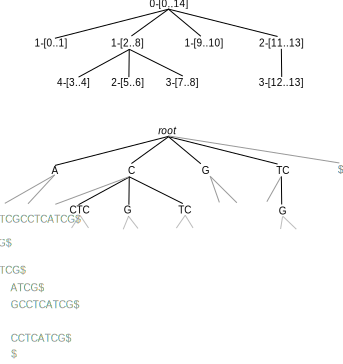
\includegraphics[width=\textwidth]{../figures/lcpintervaltree}
   \caption{LCP interval tree (top) and suffix tree (bottom).}\label{fig:enhancedsuffixarraytree}
\end{subfigure}
\caption[The suffix array, suffix tree, and lcp interval tree]{The suffix array, suffix tree, and lcp interval tree of a string ACCTCGCCTCATCG\$. Note that internal nodes (black) in suffix tree correspond to the nodes in lcp interval tree (Figure~\ref{fig:enhancedsuffixarraytree}). The singleton nodes (not shown in the image) than correspond to the leaf nodes (grey) in the suffix tree.}\label{fig:enhancedsuffixarray}
\end{figure}
The lcp-interval has an important property to the $k$-mer counting problem. An $\ell$-interval $[i..j]$ represents a string of length $\ell$ occurring $j - i + 1$ times in $S$~\cite{tallymer}. To count the $k$-mer occurrence counts, we need to read the occurrence counts from the lcp-interval tree.

We can compute the $k$-mer histogram $H_k$ using the algorithm for enumeration lcp-interval tree nodes. The algorithm~\cite{enhancedsuffixarrays} traverses the tree in the bottom up order, i.e\ a node is enumerated only after all nodes in its subtree have been enumerated.

We start with processing the singleton intervals $[i..i]$. The singleton interval $[i..i]$ corresponds to the suffix $S_{suftab[i]}$. Let $d$ be the lcp-value of the parent node of the interval $[i..i]$, $S[suftab[i]..suftab[i]+k-1]$ is a $k$-mer occurring exactly once in $S$ if and only if $d < k$ and $suftab[i]+k < n$. We increment $H_k[1]$ by one for each interval satisfying these conditions.

Then we process the other $\ell$-intervals $[i..j]$, (except the root node). Again, let $d$ be the lcp-value of the parent of interval $[i..j]$, $S[suftab[j]..suftab[j] + k - 1]$ is a $k$-mer occurring exactly $j - i + 1$ times in $S$ if and only if $d < k \leq \ell$. We increment $H_k[j-i+1]$ by one for each interval satisfying this condition.

One of the advantages of this approach is that we can compute $H_k$ for different $k$ at once --- at each step we increment specific positions in all corresponding histograms $H_k$ for each $k$ we are interested. This approach is a core of method used in Tallymer~\cite{tallymer}, but the suffix arrays are used also in other tools~\cite{jellyfish}.

\todo{ked bude cas, spomenut compressed suffix arrays}
